\documentclass[10pt]{article}
\textwidth 16.5cm
\textheight 23.5cm
\oddsidemargin 0pt
\topmargin -3cm
% \usepackage{epsf}

% Draft watermark
\usepackage[
stamp = true,
firstpageonly = true
]{draftwatermark}

% Font and formatting
\usepackage[default]{lato}
\usepackage[skip=3pt]{parskip}
\usepackage{titlesec}
\titlespacing{\paragraph}{0pt}{*1}{*2}


% Writing maths
\usepackage{
    amsmath, % aligns, equations, etc.
    amsfonts, % blackboard bold, etc.
    bbm, % blackboard bold for numbers.
}

% Figures
\usepackage{graphicx}
\usepackage{floatrow}
\floatsetup[table]{capposition=top}
\newcommand*{\figuretitle}[1]{%
    {\centering%   <--------  will only affect the title because of the grouping (by the
    \textbf{#1}%              braces before \centering and behind \medskip). If you remove
    \par\medskip}%            these braces the whole body of a {figure} env will be centered.
}

% Boxes
\usepackage{tcolorbox}
\definecolor{edi-dark-purple}{rgb}{0.4882812,0.046875,0.4296875}
\definecolor{edi-light-purple}{rgb}{0.9453125,0.8359375,0.9140625}

% References
\usepackage[
    colorlinks,
    linkcolor=black,
    citecolor=edi-dark-purple, 
    urlcolor=edi-dark-purple,
    breaklinks = true
]{hyperref}
\usepackage{xurl}


% Acronyms
\usepackage[acronym, toc]{glossaries-extra}

\setabbreviationstyle[acronym]{long-short}
\glssetcategoryattribute{acronym}{nohyperfirst}{true}
\renewcommand*{\glsdonohyperlink}[2]{%
 {\glsxtrprotectlinks \glsdohypertarget{#1}{#2}}}

 \newacronym{bfo}{BFO}{Border Force Officer}
 \newacronym[plural=SLAs, firstplural=Service Level Agreements]{sla}{SLA}{Service Level Agreement}
 \newacronym[plural=eGates, firstplural=electronic passport Gates]{egate}{eGate}{electronic passport Gate}
 \newacronym[plural=KPIs, firstplural=Key Performance Indicators]{kpi}{KPI}{Key Performance Indicator}

% Inline comments from Jacob and Bella
\usepackage{xcolor}
\usepackage[draft,inline,nomargin,index]{fixme}
\fxsetup{theme=color,mode=multiuser}
\FXRegisterAuthor{jb}{ajb}{\color{blue} JB}
\FXRegisterAuthor{bd}{abd}{\color{red} BD}

\title{Planning for Future Demand on Border Operations\\ at Edinburgh Airport (High-Level Summary)}
 \author{Isabella Deutsch and Jacob R. Bradley}
 \date{}


\begin{document}
\maketitle

\vspace{-15pt}
\paragraph{Introduction}
Edinburgh Airport has requested an investigation into the need for further construction of \glspl{egate} to support border force operations. This document provides an overview of results from the longer ten-page report of the same name. 

\paragraph{Recommendations}
We propose a schedule for \gls{egate} construction that sees no fewer than 14 \glspl{egate} available by 2023, 18 by 2024, 21 by 2025, 26 by 2026, and 30 by 2027. From a baseline of 10 \glspl{egate} currently available, this entails a 200\% increase spread approximately evenly over the five year period in question. We also strongly recommend that the airport pursue measures to increase \gls{egate} usage via increasing eligibility and uptake, in line with the 2025 UK Border Strategy. Summaries of our conclusions are given below and expanded upon in the long-form report.
\begin{tcolorbox}[
colframe=edi-dark-purple,
colback=edi-light-purple,
fonttitle=\bfseries,
title = {Summary of Recommendations and Conclusions}]
\begin{enumerate}

    \item \textbf{Building four \glsxtrshortpl{egate} per year can keep \glsxtrshort{egate} queue \glsxtrshortpl{kpi} within appropriate levels.}\\
    \item \textbf{Regardless of new \glsxtrshortpl{egate}, long desk queues pose a serious risk until \glsxtrshort{egate} usage increases.}\\
    \item \textbf{Effective \glsxtrshort{egate} usage may be achieved by expanded eligibility or by increased uptake.}\\
    \item \textbf{Lower-than-recommended \glsxtrshort{egate} construction will impact queue lengths before wait times.}\\
\end{enumerate}
\end{tcolorbox}

\paragraph{Overview of Results}
We have developed a simulation framework for  the central recommendation scenario 
\begin{figure}[!h]
    \centering
    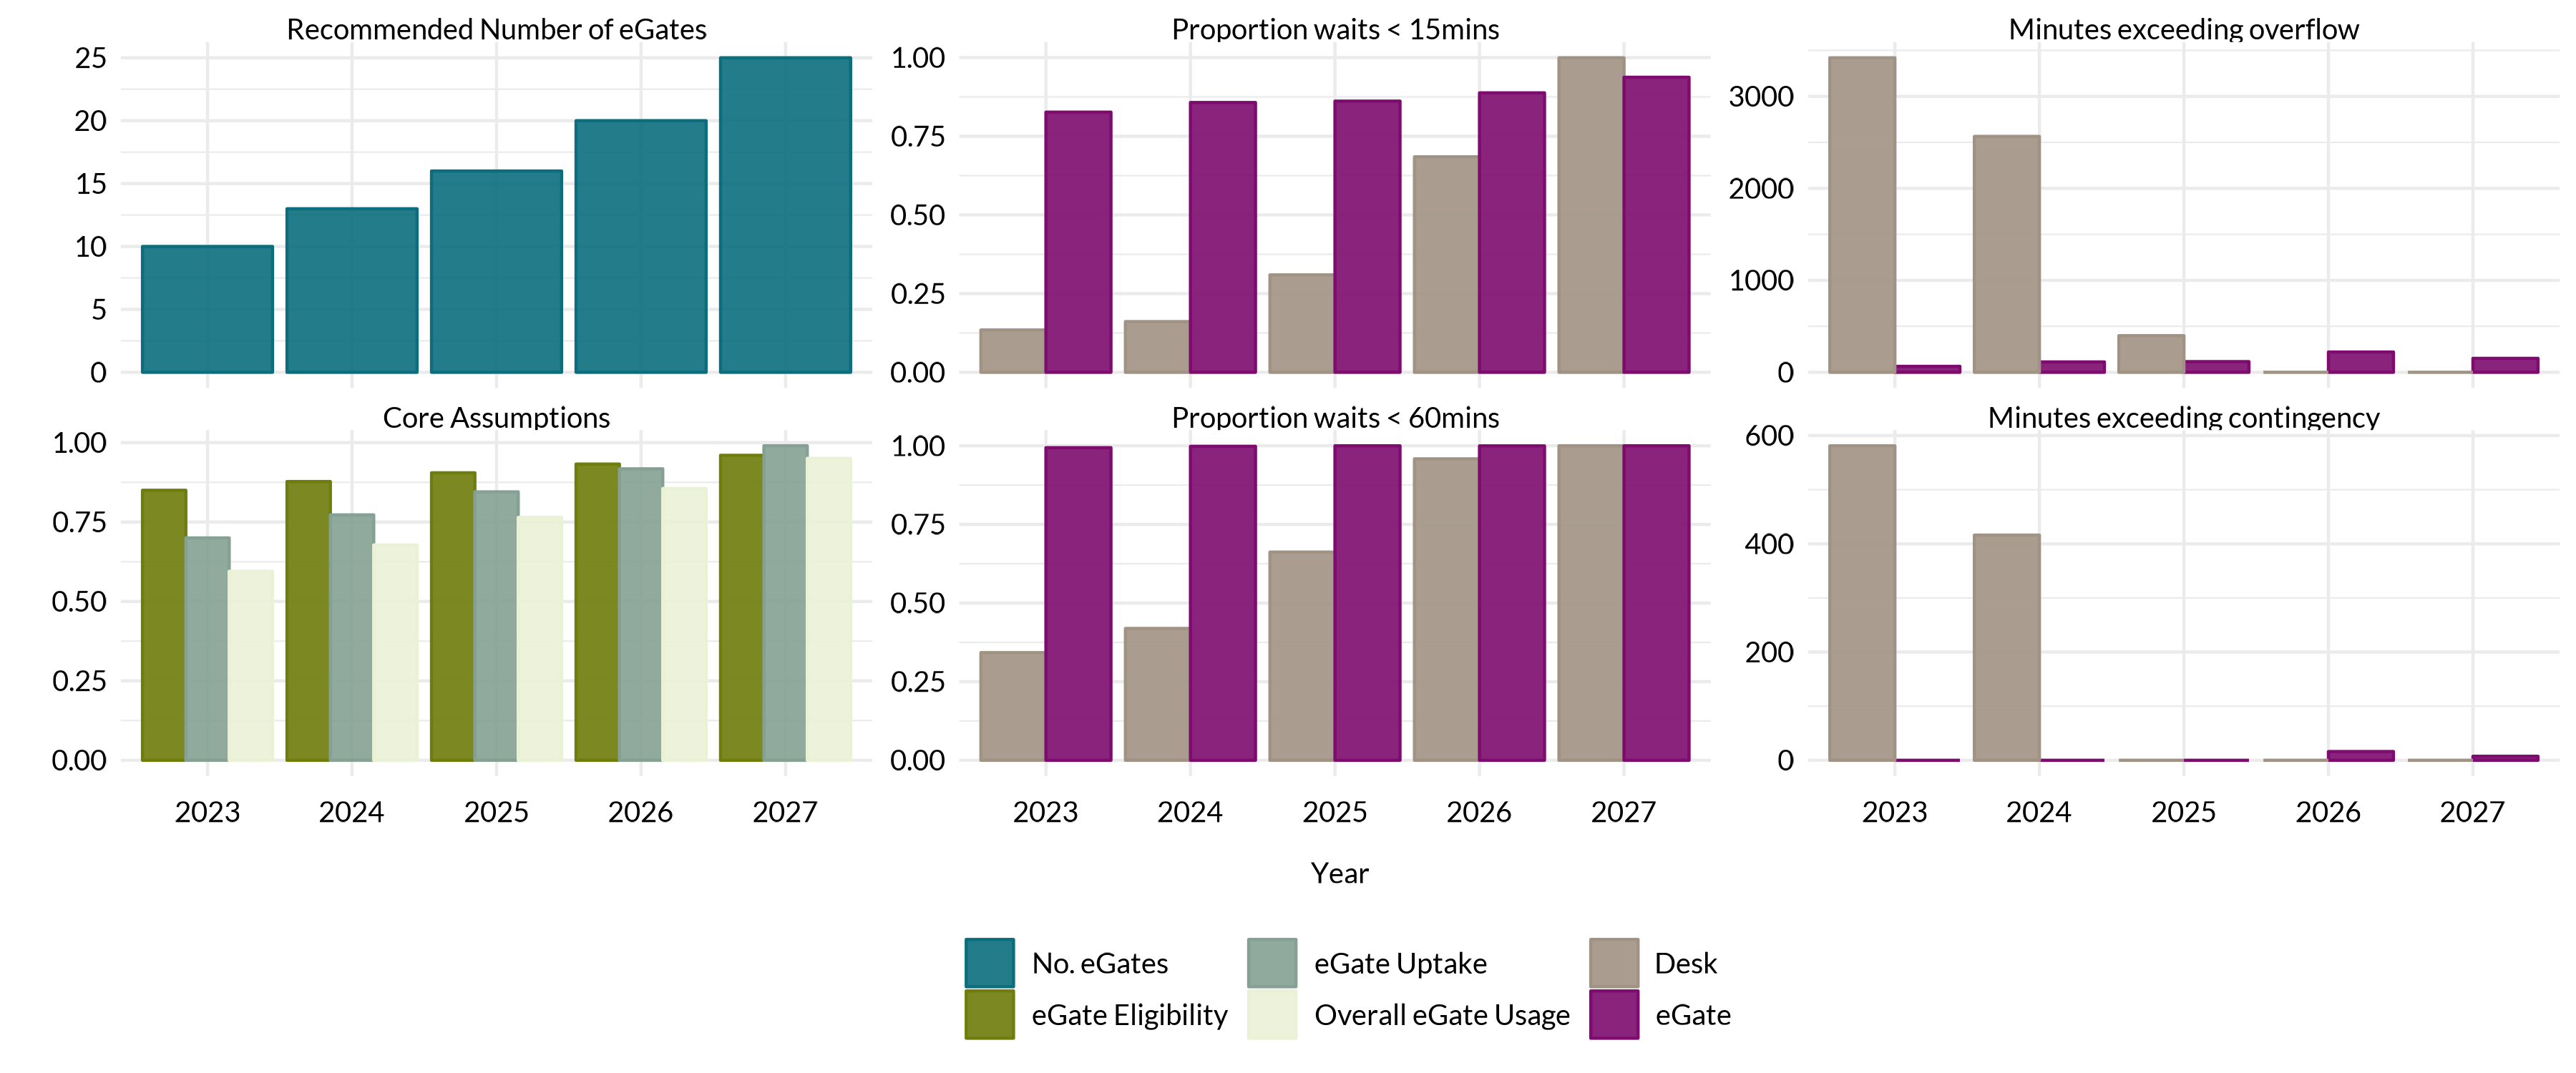
\includegraphics[width=\textwidth]{figures/core_rec_fig.png}
     \caption{Recommended \gls{egate} construction schedule, alongside usage assumptions and \glsxtrshort{kpi} summaries.} \label{fig:core_rec_fig}
\end{figure}

\end{document}